\begin{abox}
	Electronics-Problems
	\end{abox}
\begin{enumerate}
	\item Calculate values of $V_{1}$ and $V_{2}$ across $4 \Omega$ and $5 \Omega$ resistor by KVL.
	\begin{figure}[H]
		\centering
		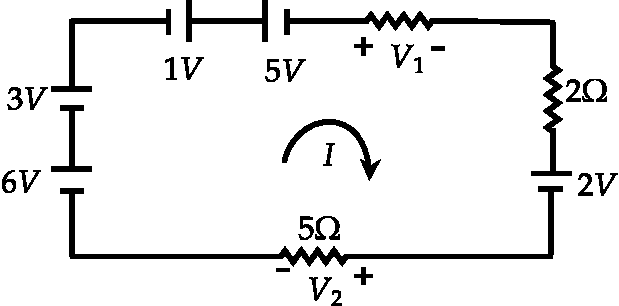
\includegraphics[height=3cm,width=6cm]{Ep-2}
	\end{figure}
	\begin{answer}
		\begin{align*}
		\text { Applying KVL }\\
		6+3+1-5-4 I-2 I-.2-5 I&=0\\
		3=111, \mathrm{I}&=\frac{3}{11} \mathrm{Amp}\\
		\mathrm{V}_{\mathrm{1}}=4 \mathrm{I}=4 \times \frac{3}{11} \mathrm{~V}&=\frac{12}{11} \text { volt }\\
		\mathrm{V}_{2}=-5 \mathrm{I}=-5 \times \frac{3}{11}&=-\frac{15}{11} \text { volt }
		\end{align*}
	\end{answer}
	\item Calculate $\mathrm{V}_{\mathrm{AB}}$ in the given circuit
	\begin{figure}[H]
		\centering
		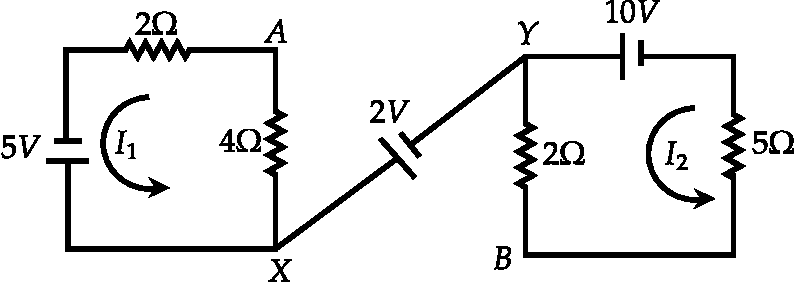
\includegraphics[height=2.8cm,width=7.5cm]{Ep-3}
	\end{figure}
	\begin{answer}
		\begin{align*}
		\mathrm{KVL} &\text { at loop 1: (Left loop) }\\
		-4 I_{1}-2 I_{1}+5&=0, \quad I_{1}=5 / 6 A m p\\
		\text { KVL at loop 2: }&\text{(Right loop) }\\
		10-2 I_{2}-5 I_{2}&=0\\
		\mathrm{I}_{2}=\frac{10}{7} \mathrm{Amp}, \mathrm{V}_{\mathrm{AB}}&=\mathrm{V}_{\mathrm{AX}}+\mathrm{V}_{\mathrm{XY}}+\mathrm{V}_{\mathrm{YB}}\\
		=-\frac{5}{6} \times 4+2+2 \times \frac{10}{7}&=-\frac{20}{6}+2+\frac{20}{7}=\frac{32}{21} V_{A B}=1.53 \text { Volt }
		\end{align*}
	\end{answer}
	\item The value of $I_{1}$ in the circuit is
	\begin{figure}[H]
		\centering
		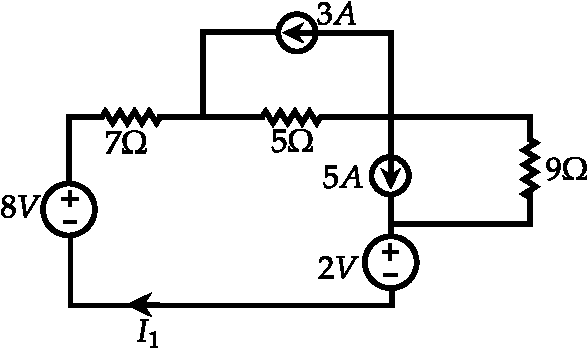
\includegraphics[height=3cm,width=5cm]{Ep-4}
	\end{figure}
	\begin{answer}$\left. \right. $
		The circuit can be redrawn in the form of voltage source as [Current $\rightarrow$ voltage source]
			\begin{figure}[H]
			\centering
			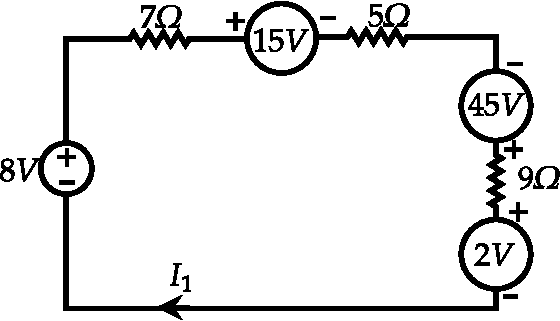
\includegraphics[height=3cm,width=5.3cm]{Ep-5}
		\end{figure}
		\begin{align*}
		\text { Applying KVL }\\
		8-7 I-15-5 I+45-9 I-2 V&=0\\
		53-17-21 \mathrm{I}=0, \quad \mathrm{I}&=\frac{36}{21} \mathrm{I}=1.71
		\end{align*}
	\end{answer}
	\item Calculate the values of $\mathrm{V}_{1}$ and $\mathrm{V}_{2}$ by $\mathrm{KCL}$ :
	\begin{figure}[H]
		\centering
		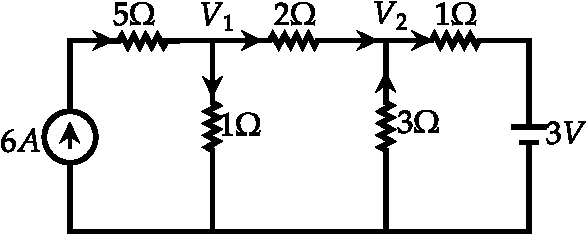
\includegraphics[height=2.5cm,width=6cm]{Ep-6}
	\end{figure}
	\begin{answer}
		\begin{align}
		\text { Applying } \mathrm{KCL} \text { at node } 1: 6&=\frac{V_{1}}{1}+\frac{V_{1}-V_{2}}{2}\label{EP-1}\\
		\mathrm{KCL} \text { at node (2) : } \frac{3-V_{2}}{1}&=\frac{V_{2}}{3}+\frac{V_{2}-V_{1}}{2}\label{EP-2}\\
		\text { By solving equation  }&\text{(\ref{EP-1}) and (\ref{EP-2});}\notag\\
		\text { We get } V_{1}&=5 \mathrm{~V} \text { and } \mathrm{V}_{2}=3 \mathrm{~V}\notag
		\end{align}
	\end{answer}
	\item Obtain single current source for network shown
	\begin{figure}[H]
		\centering
		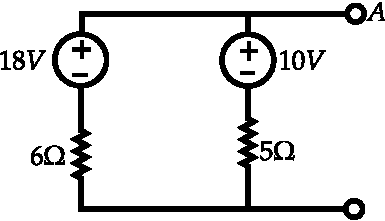
\includegraphics[height=2.5cm,width=4.4cm]{Ep-7}
	\end{figure}
	\begin{answer}
	\begin{figure}[H]
		\centering
		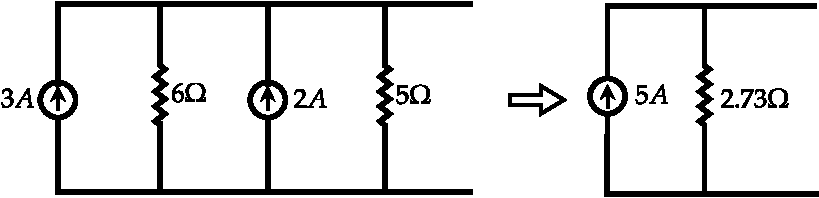
\includegraphics[height=2.5cm,width=9cm]{Ep-8}
	\end{figure}
	\end{answer}
	\item Convert given circuit into a single voltage source
	\begin{figure}[H]
		\centering
		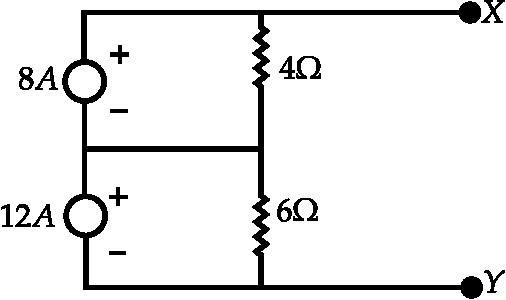
\includegraphics[height=3cm,width=5cm]{Ep-9}
	\end{figure}
	\begin{answer}$\left. \right. $\\
		\begin{figure}[H]
			\centering
			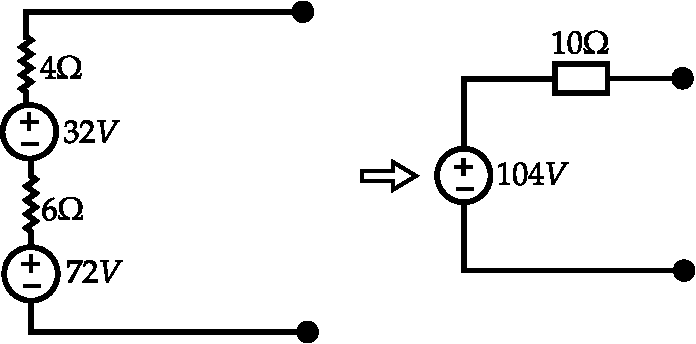
\includegraphics[height=3cm,width=6cm]{Ep-10}
		\end{figure}
	\end{answer}
	
	
	
	
	
	
	
	
	
	
	
	
	
	
	
	
\end{enumerate}